% Gabarit pandoc des corrigés publiés (brut et guidé). Contenu sans marque ni nom de site.
% Compilation : lualatex (latexmk -lualatex).
% Le Markdown reste la source unique : ne pas éditer ce fichier .tex à la main.
\documentclass[11pt,a4paper]{article}

% --- Moteur, polices (Latin Modern) et langue ---------------------------------
\usepackage{iftex}
\ifLuaTeX\else\errmessage{Ce document se compile avec lualatex}\fi
\usepackage{amsmath,amssymb,mathtools}
\usepackage{fontspec}
% mathrm=sym : \mathrm prend ses glyphes dans la police mathématique (ℓ, μ, Ω), comme KaTeX.
\usepackage[math-style=TeX,bold-style=TeX,mathrm=sym]{unicode-math}
% Repli pour les glyphes absents de Latin Modern (indices et exposants Unicode,
% flèches, filets des schémas en texte, symboles) : DejaVu, puis Latin Modern Math
% (ℓ, lettres mathématiques Unicode des légendes).
\directlua{
  luaotfload.add_fallback("repliTexte", {"DejaVuSerif:mode=harf;", "DejaVuSans:mode=harf;", "file:latinmodern-math.otf:mode=harf;"})
  luaotfload.add_fallback("repliMono", {"DejaVuSansMono:mode=harf;", "DejaVuSans:mode=harf;", "file:latinmodern-math.otf:mode=harf;"})
}
\setmainfont{Latin Modern Roman}[RawFeature={fallback=repliTexte}]
\setsansfont{Latin Modern Sans}[RawFeature={fallback=repliTexte}]
\setmonofont{Latin Modern Mono}[RawFeature={fallback=repliMono}]
\setmathfont{Latin Modern Math}
\usepackage[french]{babel}
\frenchsetup{SmallCapsFigTabCaptions=false}

% --- Mise en page --------------------------------------------------------------
\usepackage[a4paper,margin=2.2cm,headheight=14pt,footskip=1.2cm]{geometry}
\usepackage{microtype}
\setlength{\emergencystretch}{4em}
\tolerance=1500
\setlength{\parindent}{0pt}
\setlength{\parskip}{0.55\baselineskip plus 2pt minus 1pt}
\usepackage{xcolor}
% Gris nommés : babel-french rend « ! » actif dans le document.
\definecolor{gris2}{gray}{0.98}
\definecolor{gris3}{gray}{0.97}
\definecolor{gris5}{gray}{0.95}
\definecolor{gris35}{gray}{0.65}
\definecolor{gris40}{gray}{0.60}
\definecolor{gris45}{gray}{0.55}
\definecolor{gris50}{gray}{0.50}
\definecolor{gris55}{gray}{0.45}
\definecolor{gris60}{gray}{0.40}
\definecolor{gris65}{gray}{0.35}
\definecolor{gris70}{gray}{0.30}
\definecolor{gris80}{gray}{0.20}
\definecolor{gris85}{gray}{0.15}
\usepackage{graphicx}
\usepackage{float}
\usepackage{caption}
\captionsetup{font=small,labelformat=empty,justification=centering}
\usepackage{booktabs,longtable,array,multirow,calc}
\usepackage{siunitx}
\sisetup{locale=FR}
\usepackage[version=4]{mhchem}
\usepackage{listings}
\usepackage{fancyhdr}
\usepackage{lastpage}
\usepackage[most]{tcolorbox}
\usepackage{enumitem}
\setlist{nosep,leftmargin=*,topsep=2pt}
\usepackage[hidelinks,unicode]{hyperref}
\usepackage{bookmark}
\hypersetup{pdftitle={Mines-Ponts PSI — Physique 1 2026},pdfauthor={Rédigé par IA},pdfcreator={LaTeX},pdfsubject={Corrigé brut}}
\usepackage{xurl}

% --- Pandoc : listes, tableaux, figures ----------------------------------------
\providecommand{\passthrough}[1]{#1}
\providecommand{\tightlist}{\setlength{\itemsep}{0pt}\setlength{\parskip}{0pt}}

\makeatletter
\def\maxwidth{\ifdim\Gin@nat@width>\linewidth\linewidth\else\Gin@nat@width\fi}
\def\maxheight{\ifdim\Gin@nat@height>0.55\textheight 0.55\textheight\else\Gin@nat@height\fi}
\makeatother
\setkeys{Gin}{width=\maxwidth,height=\maxheight,keepaspectratio}
\setcounter{secnumdepth}{-\maxdimen}
\providecommand{\pandocbounded}[1]{#1}
\usepackage{longtable,booktabs,array}

% --- Code (listings) -----------------------------------------------------------
\lstset{
  basicstyle=\ttfamily\small,
  columns=fullflexible,
  keepspaces=true,
  breaklines=true,
  breakatwhitespace=false,
  postbreak=\mbox{\textcolor{gris50}{$\hookrightarrow$}\space},
  frame=single,
  rulecolor=\color{gris35},
  framesep=4pt,
  xleftmargin=5pt,xrightmargin=5pt,
  backgroundcolor=\color{gris3},
  keywordstyle=\bfseries,
  commentstyle=\color{gris65},
  stringstyle=\color{gris80},
  showstringspaces=false,
  tabsize=4,
  extendedchars=true,
  aboveskip=6pt,belowskip=6pt,
}

% --- Macros des corrigés (KaTeX ↔ LaTeX) ---------------------------------------
% Les corrigés sont écrits pour KaTeX : on définit ici ce que KaTeX connaît et
% que LaTeX n'a pas, sans jamais retoucher le Markdown.
\providecommand{\R}{\mathbb{R}}
\providecommand{\N}{\mathbb{N}}
\providecommand{\Z}{\mathbb{Z}}
\providecommand{\Q}{\mathbb{Q}}
\providecommand{\C}{\mathbb{C}}
\providecommand{\dd}{\mathrm{d}}
\providecommand{\llbracket}{\lBrack}
\providecommand{\rrbracket}{\rBrack}
\providecommand{\lBrace}{\lbrace}
\providecommand{\rBrace}{\rbrace}
\providecommand{\Box}{\square}
\providecommand{\Diamond}{\lozenge}
\providecommand{\varnothing}{\emptyset}
\providecommand{\argmax}{\operatorname*{arg\,max}}
\providecommand{\argmin}{\operatorname*{arg\,min}}
\renewcommand{\leq}{\leqslant}
\renewcommand{\geq}{\geqslant}

% Équation hors texte : réduite à la largeur de la ligne si elle déborde.
\newsavebox{\boiteequation}
\newcommand{\equationajustee}[1]{%
  \sbox{\boiteequation}{$\displaystyle #1$}%
  \ifdim\wd\boiteequation>\linewidth
    \[\resizebox{\linewidth}{!}{\usebox{\boiteequation}}\]%
  \else
    \[#1\]%
  \fi}

% --- Encadrés pédagogiques (sobres, lisibles en noir et blanc) -----------------
\tcbset{
  encadre/.style={
    enhanced,breakable,sharp corners,
    colback=white,colframe=gris55,
    boxrule=0.4pt,leftrule=2.2pt,
    left=6pt,right=6pt,top=3pt,bottom=3pt,
    before skip=6pt,after skip=6pt,
    fonttitle=\bfseries\small,coltitle=black,
    attach title to upper,after title={\quad},
    parbox=false,
  }
}
\newtcolorbox{indication}[1]{encadre,colframe=gris45,colback=gris2,title={Indication~#1}}
\newtcolorbox{methode}{encadre,colframe=gris70,title={Méthode}}
\newtcolorbox{piege}{encadre,colframe=gris85,boxrule=0.8pt,leftrule=2.2pt,title={Piège}}
\newtcolorbox{jury}{encadre,colframe=gris60,colback=gris5,title={Jury}}
\newtcolorbox{encadrenote}{encadre,colframe=gris40}

% --- Titres de section ---------------------------------------------------------
\usepackage{titlesec}
\titleformat{\section}{\Large\bfseries}{}{0pt}{}
\titleformat{\subsection}{\large\bfseries}{}{0pt}{}
\titleformat{\subsubsection}{\normalsize\bfseries}{}{0pt}{}
\titlespacing*{\section}{0pt}{14pt plus 4pt minus 2pt}{6pt}
\titlespacing*{\subsection}{0pt}{10pt plus 3pt minus 2pt}{4pt}
\titlespacing*{\subsubsection}{0pt}{8pt plus 2pt minus 2pt}{2pt}

% --- En-tête et pied de page ---------------------------------------------------
\pagestyle{fancy}
\fancyhf{}
\fancyhead[L]{\small\textsc{Corrigé brut} · Mines-Ponts PSI}
\fancyhead[R]{\small Physique 1 2026}
\fancyfoot[L]{\footnotesize Corrigé rédigé par IA, non officiel}
\fancyfoot[R]{\footnotesize \thepage\,/\,\pageref*{LastPage}}
\renewcommand{\headrulewidth}{0.4pt}
\renewcommand{\footrulewidth}{0pt}
\fancypagestyle{plain}{\fancyhf{}\fancyfoot[R]{\footnotesize \thepage\,/\,\pageref*{LastPage}}\fancyfoot[L]{\footnotesize Corrigé rédigé par IA, non officiel}\renewcommand{\headrulewidth}{0pt}}

\begin{document}
\thispagestyle{plain}
\begin{center}
  {\small\scshape Corrigé brut}\par\smallskip
  {\LARGE\bfseries Mines-Ponts PSI — Physique 1 2026\par}\medskip
  {\large Mines-Ponts · PSI · Physique 1 · 2026\par}
\end{center}
\vspace{2pt}\hrule\vspace{8pt}

\emph{Corrigé rédigé par IA, non officiel. Signalez toute erreur.}

Sujet : « Autour de jets d'eau ». Durée 3 h, calculatrice interdite. Données : \(\mu=10^3\ \mathrm{kg\cdot m^{-3}}\) et \(g=10\ \mathrm{m\cdot s^{-2}}\).

Dans les parties I à III, les pressions sont des surpressions (écart à la pression atmosphérique). Les valeurs numériques sont données avec un chiffre significatif.

\hypertarget{i.-bilans-de-quantituxe9-de-mouvement-et-duxe9nergie-muxe9canique}{%
\section{I. Bilans de quantité de mouvement et d'énergie mécanique}\label{i.-bilans-de-quantituxe9-de-mouvement-et-duxe9nergie-muxe9canique}}

\hypertarget{question-1}{%
\subsection{Question 1}\label{question-1}}

\textbf{Système fermé.} On note \(\delta m_e\) la masse de fluide qui traverse la section d'entrée entre \(t\) et \(t+\mathrm dt\), et \(\delta m_s\) celle qui traverse la section de sortie pendant la même durée. On désigne par les mêmes symboles les tranches de fluide correspondantes.

On définit le système fermé \(S_F\) comme l'ensemble des particules contenues à l'instant \(t\) dans \(\Sigma(t)\) ou dans la tranche \(\delta m_e\) qui va entrer.

À l'instant \(t+\mathrm dt\), ces mêmes particules occupent le volume \(\Sigma\) et la tranche \(\delta m_s\) qui vient de sortir :

\equationajustee{S_F(t)=\Sigma(t)\cup\delta m_e}

\equationajustee{S_F(t+\mathrm dt)=\Sigma(t+\mathrm dt)\cup\delta m_s}

\textbf{Conservation de la masse.} La masse de \(S_F\) est constante. L'écoulement est permanent et la surface de contrôle fixe, donc la masse contenue dans \(\Sigma\) ne dépend pas du temps. Il en résulte \(\delta m_e=\delta m_s\), et, le débit volumique étant \(Q\) :

\equationajustee{\delta m_e=\delta m_s=\mu Q\,\mathrm dt}

\textbf{Variation de quantité de mouvement.} Les vitesses étant uniformes sur les sections d'entrée et de sortie,

\equationajustee{\mathrm d\vec p=\big[\vec p_\Sigma(t+\mathrm dt)+\mu Q\,\mathrm dt\,\vec v_s\big]-\big[\vec p_\Sigma(t)+\mu Q\,\mathrm dt\,\vec v_e\big].}

Pour la même raison de permanence, \(\vec p_\Sigma(t+\mathrm dt)=\vec p_\Sigma(t)\). Donc

\equationajustee{\boxed{\mathrm d\vec p=\mu Q\,(\vec v_s-\vec v_e)\,\mathrm dt}}

\textbf{Relation demandée.} \(S_F\) est un système fermé (déformable). Le théorème de la résultante cinétique, ou théorème du centre d'inertie, dans le référentiel galiléen du laboratoire s'écrit \(\mathrm d\vec p/\mathrm dt=\vec R_{\rm ext}\). On en déduit

\equationajustee{\boxed{\mu Q\,(\vec v_s-\vec v_e)=\vec R_{\rm ext}}}

\hypertarget{question-2}{%
\subsection{Question 2}\label{question-2}}

On garde le même système fermé. L'énergie cinétique est additive et les vitesses sont uniformes sur les sections :

\equationajustee{\begin{aligned}
\mathrm dE_c&=\big[E_{c,\Sigma}(t+\mathrm dt)+\tfrac12\mu Q\,\mathrm dt\,v_s^2\big]-\big[E_{c,\Sigma}(t)+\tfrac12\mu Q\,\mathrm dt\,v_e^2\big]\\
&=\tfrac12\mu Q\,(v_s^2-v_e^2)\,\mathrm dt,
\end{aligned}}

car \(E_{c,\Sigma}\) ne dépend pas du temps en régime permanent.

Le théorème de l'énergie cinétique appliqué, dans le référentiel galiléen du laboratoire, au système fermé \textbf{déformable} \(S_F\) s'écrit \(\mathrm dE_c/\mathrm dt=P_{\rm int}+P_{\rm ext}\). Donc

\equationajustee{\boxed{\tfrac12\mu Q\,(v_s^2-v_e^2)=P_{\rm int}+P_{\rm ext}}}

\(P_{\rm int}\) contient la puissance des forces intérieures, c'est-à-dire celle des forces de viscosité : les forces de pression intérieures ne travaillent pas pour un fluide incompressible.

\hypertarget{ii.-lance-uxe0-incendie}{%
\section{II. Lance à incendie}\label{ii.-lance-uxe0-incendie}}

\hypertarget{question-3}{%
\subsection{Question 3}\label{question-3}}

Prenons comme surface de contrôle la portion de tuyau entre les sections droites passant par deux points quelconques \(M\) et \(M'\). La paroi est imperméable. L'écoulement est permanent, donc la masse contenue est constante ; le fluide est incompressible, donc le débit volumique entrant égale le débit sortant.

La vitesse étant tangente au tuyau et uniforme sur la section d'aire \(A\) :

\equationajustee{Q=v(M)\,A=v(M')\,A .}

\(A\) étant constante le long du tuyau, \textbf{\(v(M)=v=Q/A\) est la même en tout point du tuyau}. Seule la norme est constante : le vecteur \(\vec v=v\,\hat t(M)\) tourne avec le tuyau.

\hypertarget{question-4}{%
\subsection{Question 4}\label{question-4}}

\textbf{Convention.} Le texte définit \(\vec T(M)=T\hat t(M)\) comme l'action de l'amont sur l'aval. La figure 3 dessine pourtant \(-\vec T_1\) en \(M_1\) et \(+\vec T_2\) en \(M_2\), c'est-à-dire des forces qui tirent la portion vers l'extérieur.

On retient la convention de la figure, qui est celle d'une tension (\(T>0\) : tuyau tendu). La partie aval exerce \(+T\hat t\) sur la partie amont et la partie amont exerce \(-T\hat t\) sur la partie aval. Avec la convention littérale du texte, on obtiendrait le même résultat au signe près.

\textbf{Système.} On étudie le système formé de la paroi du tuyau entre \(M_1\) et \(M_2\) et de l'eau qu'elle contient. La paroi est immobile : sa quantité de mouvement est constante. L'eau contenue est le système ouvert de la question 1, en écoulement permanent. La relation de la question 1 s'applique donc à l'ensemble, \(\vec R_{\rm ext}\) désignant la résultante des actions extérieures à la paroi et à l'eau.

\textbf{Actions extérieures}, dans le plan horizontal :

\begin{itemize}
\tightlist
\item
  tension en \(M_1\) : \(-T(M_1)\,\hat t(M_1)\) ; tension en \(M_2\) : \(+T(M_2)\,\hat t(M_2)\) ;
\item
  surpression de l'eau amont sur la section d'entrée : \(+pA\,\hat t(M_1)\) ;
\item
  surpression de l'eau aval sur la section de sortie : \(-pA\,\hat t(M_2)\) ;
\item
  sol mouillé sans frottement : réaction verticale qui compense le poids ; atmosphère : résultante nulle.
\end{itemize}

\begin{figure}[H]
\centering
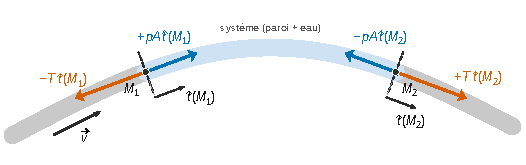
\includegraphics{figures/q04-bilan-tuyau.pdf}
\caption*{Figure 1 --- bilan sur la portion de tuyau entre M₁ et M₂ : les tensions
tirent vers l'extérieur, les surpressions poussent vers l'intérieur}
\end{figure}

D'après la question 3, \(\vec v_e=v\hat t(M_1)\) et \(\vec v_s=v\hat t(M_2)\). La relation de la question 1 donne alors

\equationajustee{\mu Qv\,\big(\hat t(M_2)-\hat t(M_1)\big)=-T(M_1)\hat t(M_1)+T(M_2)\hat t(M_2)+pA\,\hat t(M_1)-pA\,\hat t(M_2),}

soit

\equationajustee{\big[T(M_2)-\mu Qv-pA\big]\hat t(M_2)=\big[T(M_1)-\mu Qv-pA\big]\hat t(M_1).}

Les vecteurs \(\hat t(M_1)\) et \(\hat t(M_2)\) ne sont pas colinéaires : les deux coefficients sont nuls. Donc

\equationajustee{T(M_1)=T(M_2)=T}

\equationajustee{\boxed{T=\mu Qv+pA}}

La tension est uniforme et positive : le tuyau est tendu, quelle que soit sa disposition.

\hypertarget{question-5}{%
\subsection{Question 5}\label{question-5}}

\textbf{Vitesse d'éjection.} Par conservation du débit, \(Q=vA=v_sA_s\), donc

\equationajustee{\boxed{v_s=\frac{A}{A_s}\,v}}

\textbf{Force du pompier.} Le système est la lance et l'eau qu'elle contient. La section d'entrée a pour aire \(A\), la surpression y vaut \(p\) et la vitesse \(v\hat t_s\). La section de sortie a pour aire \(A_s\), la surpression y est nulle (jet libre à l'air) et la vitesse vaut \(v_s\hat t_s\).

Actions extérieures, projetées sur \(\hat t_s\) (le poids est compensé) :

\begin{itemize}
\tightlist
\item
  tension du tuyau amont : \(-T\hat t_s\), avec \(T=\mu Qv+pA\) (question 4) ;
\item
  surpression de l'eau amont sur la section d'entrée : \(+pA\,\hat t_s\) ;
\item
  action du pompier : \(\vec F\).
\end{itemize}

La relation de la question 1 donne

\equationajustee{\mu Q\,(v_s-v)\,\hat t_s=-(\mu Qv+pA)\,\hat t_s+pA\,\hat t_s+\vec F,}

d'où

\equationajustee{\boxed{\vec F=\mu Q\,\vec v_s=\mu Q\,v_s\,\hat t_s}}

\textbf{Sens.} Le coefficient \(\mu Qv_s\) est strictement positif, donc \(\vec F\) a le sens de \(\hat t_s\), celui du jet : \textbf{le pompier doit pousser la lance vers l'avant} (il retient le recul de la lance).

\begin{figure}[H]
\centering
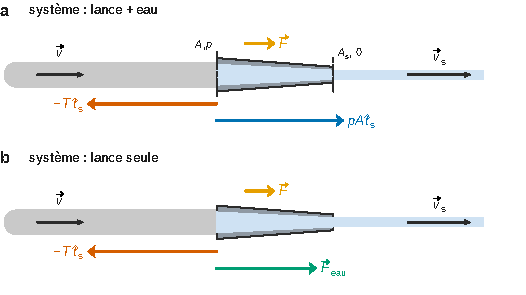
\includegraphics{figures/q05-q06-bilan-lance.pdf}
\caption*{Figure 2 --- bilans sur la lance, (a) lance et eau contenue (Q5), (b)
lance seule (Q6) ; longueurs indicatives, avec F + F\_eau = T}
\end{figure}

\hypertarget{question-6}{%
\subsection{Question 6}\label{question-6}}

On change de système : la lance seule, solide de masse négligeable en équilibre. L'action de l'eau sur la lance devient alors une action extérieure.

La lance subit la tension du tuyau \(-T\hat t_s\), l'action du pompier \(F\hat t_s\) et l'action de l'eau \(F_{\rm eau}\hat t_s\) ; l'atmosphère a une résultante nulle. L'équilibre projeté sur \(\hat t_s\) donne \(-T+F+F_{\rm eau}=0\) :

\equationajustee{\boxed{F_{\rm eau}=T-F}}

\hypertarget{question-7}{%
\subsection{Question 7}\label{question-7}}

\textbf{Bernoulli.} L'écoulement est parfait, stationnaire, incompressible et homogène entre l'entrée et la sortie de la lance, qui sont à la même altitude. Le long d'une ligne de courant, en surpressions, avec une surpression nulle dans le jet libre de sortie :

\equationajustee{\boxed{p+\tfrac12\mu v^2=\tfrac12\mu v_s^2}}

soit

\equationajustee{p=\tfrac12\mu\,(v_s^2-v^2).}

\textbf{Tension.} Avec \(v=Q/A\) et \(v_s=Q/A_s\) :

\equationajustee{\begin{aligned}
T&=\mu Qv+pA\\
&=\frac{\mu Q^2}{A}+\frac{\mu A}{2}\left(\frac{Q^2}{A_s^2}-\frac{Q^2}{A^2}\right)\\
&=\frac12\mu Q^2\frac1A\left[1+\left(\frac{A}{A_s}\right)^2\right].
\end{aligned}}

\equationajustee{\boxed{T=\frac12\mu Q^2\frac1A\,k_1}}

\equationajustee{\boxed{k_1=1+\left(\frac{A}{A_s}\right)^2}}

\textbf{Action de l'eau.} La force du pompier s'écrit avec le même préfacteur :

\equationajustee{\begin{aligned}
F&=\mu Qv_s=\frac{\mu Q^2}{A_s}\\
&=\frac12\mu Q^2\frac1A\cdot\frac{2A}{A_s}.
\end{aligned}}

Donc

\equationajustee{\begin{aligned}
F_{\rm eau}&=T-F\\
&=\frac12\mu Q^2\frac1A\left[1+\left(\frac A{A_s}\right)^2-2\frac A{A_s}\right].
\end{aligned}}

\equationajustee{\boxed{F_{\rm eau}=\frac12\mu Q^2\frac1A\,k_2}}

\equationajustee{\boxed{k_2=\left(\frac{A}{A_s}-1\right)^2}}

\textbf{Sens.} \(k_2\ge0\) : \textbf{l'eau pousse la lance vers l'avant}, dans le sens de l'écoulement (action nulle seulement si \(A_s=A\)).

\textbf{Comparaison.} \(T-F_{\rm eau}=F>0\), donc \textbf{\(F_{\rm eau}<T\)}, l'écart étant exactement la force du pompier.

Pour \(A/A_s\gg1\), \(T\) et \(F_{\rm eau}\) sont du même ordre, car \(k_1\) et \(k_2\) sont tous deux voisins de \((A/A_s)^2\).

\hypertarget{question-8}{%
\subsection{Question 8}\label{question-8}}

Conversion du débit :

\equationajustee{\begin{aligned}
Q&=600\ \mathrm{L\cdot min^{-1}}=\frac{0{,}6}{60}\ \mathrm{m^3\cdot s^{-1}}\\
&=1{,}0\times10^{-2}\ \mathrm{m^3\cdot s^{-1}}.
\end{aligned}}

Alors \(A/A_s=20\), \(k_1=401\) et \(k_2=19^2=361\). Le préfacteur vaut

\equationajustee{\frac12\mu\frac{Q^2}{A}=\frac12\times10^3\times\frac{10^{-4}}{10^{-2}}=5\ \mathrm N .}

On en déduit les deux forces :

\equationajustee{\begin{aligned}
F_{\rm eau}&=5\times361\ \mathrm N\approx1{,}8\times10^3\ \mathrm N,\\
F&=\mu Q\frac{Q}{A_s}=10^3\times10^{-2}\times20\ \mathrm N=200\ \mathrm N .
\end{aligned}}

À un chiffre significatif :

\equationajustee{\boxed{F_{\rm eau}\approx2\times10^3\ \mathrm N}}

\equationajustee{\boxed{F\approx2\times10^2\ \mathrm N}}

On trouve aussi \(T\approx2\times10^3\) N. \textbf{Vraisemblance.} Le pompier fournit l'équivalent du poids d'une masse de \(20\) kg, effort important mais humainement possible. La surpression dans le tuyau, \(p=\tfrac12\mu(v_s^2-v^2)\approx2\times10^5\) Pa, soit \(2\) bar, est elle aussi plausible.

\hypertarget{iii.-jet-deau-vertical}{%
\section{III. Jet d'eau vertical}\label{iii.-jet-deau-vertical}}

\hypertarget{question-9}{%
\subsection{Question 9}\label{question-9}}

Dans le jet libre, la surpression est nulle et les frottements de l'air sont négligés : chaque particule de fluide n'est soumise qu'à son poids. Le référentiel terrestre est supposé galiléen.

La conservation de l'énergie mécanique d'une particule, entre la sortie (vitesse \(v_s\) verticale) et le sommet du jet (vitesse nulle), donne \(\tfrac12 v_s^2=gh\) :

\equationajustee{\boxed{h=\frac{v_s^2}{2g}}}

\hypertarget{question-10}{%
\subsection{Question 10}\label{question-10}}

On applique le théorème de Bernoulli entre le réseau (surpression \(p_0\), vitesse négligeable) et la sortie (surpression nulle, vitesse \(v_{s,m}\)), à la même altitude :

\equationajustee{p_0=\tfrac12\mu v_{s,m}^2}

donc

\equationajustee{\boxed{v_{s,m}=\sqrt{\frac{2p_0}{\mu}}}}

Avec la question 9 :

\equationajustee{\boxed{h_m=\frac{v_{s,m}^2}{2g}=\frac{p_0}{\mu g}}}

\(h_m\) ne dépend ni de \(d\), ni de \(D\), ni de \(L\) : \textbf{dans ce modèle sans perte, rétrécir la sortie ne modifie pas la hauteur du jet} (seul le débit change).

Pour \(p_0=3\ \mathrm{bar}=3\times10^5\ \mathrm{Pa}\), on trouve \(v_{s,m}=\sqrt{600}\ \mathrm{m\cdot s^{-1}}\approx24\ \mathrm{m\cdot s^{-1}}\) et

\equationajustee{\boxed{h_m=\frac{3\times10^5}{10^3\times10}\ \mathrm m=3\times10^1\ \mathrm m}}

\textbf{Vraisemblance.} Une surpression de \(1\) bar équilibre environ \(10\) m d'eau : \(3\) bar correspondent bien à \(30\) m.

\hypertarget{question-11}{%
\subsection{Question 11}\label{question-11}}

\textbf{Nombres sans dimension.} \(f\) dépend du \textbf{nombre de Reynolds} \(\mathrm{Re}=\mu vD/\eta\), où \(\eta\) est la viscosité dynamique. Il dépend aussi de la \textbf{rugosité relative} \(e/D\), où \(e\) est la hauteur moyenne des aspérités de la paroi.

\textbf{Représentation graphique.} Le réseau de courbes \(f(\mathrm{Re})\) paramétré par \(e/D\), en échelles logarithmiques, est le \textbf{diagramme de Moody}. En régime laminaire, \(f=64/\mathrm{Re}\) ne dépend pas de la rugosité. En régime turbulent, \(f\) décroît lentement avec \(\mathrm{Re}\) et devient indépendant de \(\mathrm{Re}\) pour une paroi rugueuse aux grands nombres de Reynolds.

\textbf{Puissance dissipée.} Hypothèses : régime permanent, fluide incompressible, conduite horizontale de section constante, vitesse uniforme sur la section. On applique la relation de la question 2 au fluide de la conduite entre les sections de surpressions \(p_1\) et \(p_2\) :

\begin{itemize}
\tightlist
\item
  section constante : \(v_e=v_s=v\), le membre de gauche est nul ;
\item
  \(P_{\rm ext}\) se réduit à la puissance des forces de surpression sur les deux sections, \(p_1Av-p_2Av=(p_1-p_2)Q\) ;
\item
  la paroi immobile ne travaille pas, et le poids non plus (conduite horizontale) ;
\item
  \(P_{\rm int}=-P_{\rm dis}\) : seules les forces de viscosité travaillent (fluide incompressible).
\end{itemize}

Donc \(0=(p_1-p_2)Q-P_{\rm dis}\) :

\equationajustee{\boxed{P_{\rm dis}=Q\,(p_1-p_2)=\frac12\mu v^2\frac LD f\,Q}}

Cette puissance est positive puisque \(p_1>p_2\).

\hypertarget{question-12}{%
\subsection{Question 12}\label{question-12}}

\textbf{Interprétation de la perte singulière.} Il faut prendre en compte trois effets : la perte de charge régulière dans la conduite, la perte de charge singulière au rétrécissement et le changement de section, qui accélère le fluide de \(v\) à \(v_s\).

On interprète donc \(\tfrac12\mu v_s^2K\) comme une perte de \textbf{charge}, c'est-à-dire une perte de \(p+\tfrac12\mu v^2\) à la traversée du rétrécissement :

\equationajustee{\big(p_D+\tfrac12\mu v^2\big)-\big(p_d+\tfrac12\mu v_s^2\big)=\tfrac12\mu v_s^2K.}

C'est la seule lecture compatible avec la vérification demandée : sans pertes, on doit retrouver \(v_s=v_{s,m}\).

\textbf{Bilan.} On écrit le bilan de charge entre le réseau (surpression \(p_0\), vitesse négligeable) et la sortie du rétrécissement (surpression nulle, vitesse \(v_s\)), à la même altitude. Il cumule Bernoulli au raccordement, la perte régulière dans la conduite (vitesse \(v\)) et la perte singulière au rétrécissement :

\equationajustee{p_0=\frac12\mu v_s^2+\frac12\mu v^2\frac LD f+\frac12\mu v_s^2K .}

\textbf{Débit.} La conservation du débit s'écrit \(v\,\pi D^2/4=v_s\,\pi d^2/4\), donc

\equationajustee{v=v_s\left(\frac dD\right)^2.}

Avec \(p_0=\tfrac12\mu v_{s,m}^2\) (question 10) :

\equationajustee{\boxed{v_s=\frac{v_{s,m}}{\sqrt{1+K+f\dfrac LD\left(\dfrac dD\right)^4}}}}

Si l'on néglige toutes les pertes (\(f=K=0\)), on retrouve \(v_s=v_{s,m}\) : le résultat est cohérent avec la question 10.

\textbf{Hauteur.} Par la question 9, \(h=v_s^2/(2g)\) :

\equationajustee{\boxed{h=\frac{h_m}{1+K+f\dfrac LD\left(\dfrac dD\right)^4}}}

\(K\ge0\) et \(f\ge0\), car les pertes sont dissipatives (question 11). Le dénominateur est donc au moins égal à \(1\) : \textbf{\(h\le h_m\), il est impossible d'obtenir un jet plus haut que \(h_m\).}

\hypertarget{question-13}{%
\subsection{Question 13}\label{question-13}}

Rapports utiles :

\equationajustee{\begin{aligned}
\frac LD&=\frac{25}{2{,}5\times10^{-2}}=10^3,\\
f\frac LD&=20,\\
\left(\frac dD\right)^4&=\left(4\times10^{-2}\right)^4=2{,}56\times10^{-6}.
\end{aligned}}

\textbf{Avec rétrécissement} (\(d=1\) mm, \(K=0{,}5\)). Le dénominateur vaut \(1+0{,}5+20\times2{,}56\times10^{-6}\simeq1{,}5\). Donc

\equationajustee{\begin{aligned}
h&=\frac{30}{1{,}5}\ \mathrm m=20\ \mathrm m,\\
v_s&=\frac{24{,}5}{\sqrt{1{,}5}}\ \mathrm{m\cdot s^{-1}}=20\ \mathrm{m\cdot s^{-1}},\\
v&=v_s\left(\frac dD\right)^2=20\times1{,}6\times10^{-3}\ \mathrm{m\cdot s^{-1}}=3{,}2\times10^{-2}\ \mathrm{m\cdot s^{-1}}.
\end{aligned}}

\textbf{Sans rétrécissement} (\(d=D\), donc \(v_s=v\) et pas de perte singulière). Le dénominateur vaut \(1+20=21\). Donc

\equationajustee{\begin{aligned}
h&=\frac{30}{21}\ \mathrm m\approx1{,}4\ \mathrm m,\\
v_s=v&=\frac{24{,}5}{\sqrt{21}}\ \mathrm{m\cdot s^{-1}}\approx5{,}3\ \mathrm{m\cdot s^{-1}}.
\end{aligned}}

Garder \(K=0{,}5\) dans ce cas donnerait \(h=30/21{,}5\approx1{,}4\) m : même résultat à un chiffre significatif.

\begin{longtable}[]{@{}
  >{\raggedright\arraybackslash}p{(\columnwidth - 6\tabcolsep) * \real{0.2447}}
  >{\raggedright\arraybackslash}p{(\columnwidth - 6\tabcolsep) * \real{0.1667}}
  >{\raggedright\arraybackslash}p{(\columnwidth - 6\tabcolsep) * \real{0.2736}}
  >{\raggedright\arraybackslash}p{(\columnwidth - 6\tabcolsep) * \real{0.2850}}@{}}
\toprule\noalign{}
\begin{minipage}[b]{\linewidth}\raggedright
Configuration
\end{minipage} & \begin{minipage}[b]{\linewidth}\raggedright
\(h\)
\end{minipage} & \begin{minipage}[b]{\linewidth}\raggedright
\(v_s\)
\end{minipage} & \begin{minipage}[b]{\linewidth}\raggedright
\(v\)
\end{minipage} \\
\midrule\noalign{}
\endhead
\bottomrule\noalign{}
\endlastfoot
Avec rétrécissement (\(d=1\) mm) & \(2\times10^1\) m & \(2\times10^1\ \mathrm{m\cdot s^{-1}}\) & \(3\times10^{-2}\ \mathrm{m\cdot s^{-1}}\) \\
Sans rétrécissement (\(d=D\)) & \(1\) m & \(5\ \mathrm{m\cdot s^{-1}}\) & \(5\ \mathrm{m\cdot s^{-1}}\) \\
\end{longtable}

\textbf{Explication.} En rétrécissant la sortie, on réduit fortement le débit, donc la vitesse \(v\) dans la longue conduite ; la perte de charge régulière, proportionnelle à \(v^2\), devient négligeable et la surpression du réseau est presque entièrement convertie en énergie cinétique du jet.

\hypertarget{iv.-instabilituxe9-de-rayleigh-plateau}{%
\section{IV. Instabilité de Rayleigh-Plateau}\label{iv.-instabilituxe9-de-rayleigh-plateau}}

\hypertarget{iv.a-moduxe8le}{%
\subsection{IV.A Modèle}\label{iv.a-moduxe8le}}

\hypertarget{question-14}{%
\subsection{Question 14}\label{question-14}}

La loi de Laplace, \(P_{\rm int}-P_{\rm ext}=\alpha\left(1/R_1-1/R_2\right)\), montre que \(\alpha\) est une pression (\(P\) est ici une pression) multipliée par une longueur (\(R_1\) et \(R_2\) sont des rayons) :

\equationajustee{[\alpha]=\mathrm{N\cdot m^{-2}}\cdot\mathrm m .}

\equationajustee{\boxed{\alpha\ \text{s'exprime en}\ \mathrm{N\cdot m^{-1}},\ \text{soit aussi}\ \mathrm{J\cdot m^{-2}}\ \text{ou}\ \mathrm{kg\cdot s^{-2}}}}

C'est une énergie par unité de surface, d'où \(E_p=\alpha S\).

\hypertarget{question-15}{%
\subsection{Question 15}\label{question-15}}

Le volume de la tranche, de longueur \(\lambda=2\pi/k\) (une période), est

\equationajustee{\begin{aligned}
V&=\int_{-\lambda/2}^{\lambda/2}\pi\big(R+\varepsilon\sin kz\big)^2\mathrm dz\\
&=\pi\left(R^2\lambda+0+\varepsilon^2\frac\lambda2\right),
\end{aligned}}

car \(\sin kz\) est de moyenne nulle et \(\sin^2kz\) de moyenne \(1/2\) sur une période.

L'eau étant incompressible, le volume de la tranche non perturbée se conserve : \(V=\pi R_0^2\lambda\). D'où \(R^2=R_0^2-\varepsilon^2/2\) et, au second ordre en \(\varepsilon/R_0\),

\equationajustee{\boxed{R=R_0\left(1-\frac{\varepsilon^2}{4R_0^2}\right)=R_0-\frac{\varepsilon^2}{4R_0}}}

\hypertarget{question-16}{%
\subsection{Question 16}\label{question-16}}

La dérivée \(\mathrm dr/\mathrm dz=\varepsilon k\cos kz\) est du premier ordre en \(\varepsilon\) (\(\varepsilon\ll\lambda\)). Le développement de la racine au second ordre s'écrit donc

\equationajustee{\sqrt{1+\left(\frac{\mathrm dr}{\mathrm dz}\right)^2}=1+\tfrac12\varepsilon^2k^2\cos^2kz+O(\varepsilon^4),}

et

\equationajustee{r\sqrt{1+\left(\frac{\mathrm dr}{\mathrm dz}\right)^2}=R+\varepsilon\sin kz+\frac12R\varepsilon^2k^2\cos^2kz+O(\varepsilon^3).}

On intègre sur une période, où \(\sin kz\) est de moyenne nulle et \(\cos^2kz\) de moyenne \(1/2\) :

\equationajustee{\begin{aligned}
S&=2\pi\left(R\lambda+\frac{R\varepsilon^2k^2\lambda}{4}\right)\\
&=2\pi R\lambda\left(1+\frac{k^2\varepsilon^2}{4}\right).
\end{aligned}}

On reporte \(R=R_0\big(1-\varepsilon^2/(4R_0^2)\big)\) et on ne garde que l'ordre 2 :

\equationajustee{\boxed{S=2\pi R_0\lambda\left(1+\gamma\varepsilon^2\right)}}

\equationajustee{\boxed{\gamma=\frac14\left(k^2-\frac1{R_0^2}\right)=\frac{k^2R_0^2-1}{4R_0^2}}}

\textbf{Stabilité.} L'énergie potentielle vaut \(E_p=\alpha S=2\pi\alpha R_0\lambda(1+\gamma\varepsilon^2)\), avec \(\alpha>0\).

\begin{itemize}
\tightlist
\item
  Si \(\gamma>0\), l'état non perturbé \(\varepsilon=0\) est un minimum d'énergie potentielle : il est stable.
\item
  Si \(\gamma<0\), c'est un maximum : la perturbation abaisse l'énergie et croît.
\end{itemize}

La stabilité équivaut donc à \(kR_0>1\), soit \(2\pi/\lambda>1/R_0\) :

\equationajustee{\boxed{\lambda<\lambda_\ell=2\pi R_0}}

\hypertarget{question-17}{%
\subsection{Question 17}\label{question-17}}

Au premier ordre, \(R=R_0\) et \((\mathrm dr/\mathrm dz)^2=O(\varepsilon^2)\) : les crochets des deux courbures valent \(1\). Donc

\equationajustee{\frac1{R_1}=\frac1{R_0+\varepsilon\sin kz}\simeq\frac1{R_0}-\frac{\varepsilon\sin kz}{R_0^2},}

\equationajustee{\frac1{R_2}=\frac{\mathrm d^2r}{\mathrm dz^2}=-\varepsilon k^2\sin kz .}

La loi de Laplace donne alors

\equationajustee{\begin{aligned}
\Delta P&=\alpha\left(\frac1{R_1}-\frac1{R_2}\right)\\
&=\frac\alpha{R_0}+\alpha\varepsilon\left(k^2-\frac1{R_0^2}\right)\sin kz.
\end{aligned}}

\equationajustee{\boxed{\Delta P=\frac{\alpha}{R_0}+4\alpha\gamma\,\varepsilon\sin(kz)}}

\textbf{Condition de stabilité.} Pour \(\varepsilon>0\), le rayon est maximal là où \(\sin kz=+1\) (ventres) et minimal là où \(\sin kz=-1\) (cols). L'effet est modérateur si la pression est plus forte dans les ventres que dans les cols : le fluide est alors chassé des ventres vers les cols.

Il faut donc \(4\alpha\gamma\varepsilon>0\), soit \(\gamma>0\), c'est-à-dire \(\lambda<2\pi R_0\). On retrouve le critère de la question 16.

Le terme \(-1/R_0^2\) vient de la courbure azimutale \(1/R_1\) : il est déstabilisant et domine aux grandes longueurs d'onde. Le terme \(k^2\) vient de la courbure axiale \(1/R_2\) : il est stabilisant et domine aux petites longueurs d'onde.

\begin{figure}[H]
\centering
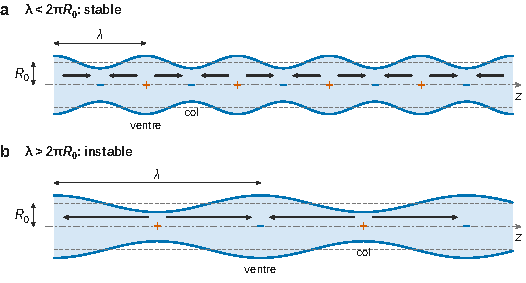
\includegraphics{figures/q17-pression-ventres-cols.pdf}
\caption*{Figure 3 --- lecture en pression du critère : « + » marque la
surpression la plus forte, les flèches le sens où le fluide est chassé}
\end{figure}

\hypertarget{question-18}{%
\subsection{Question 18}\label{question-18}}

On cherche \(\tau_h=\mu^aR_0^b\alpha^c\), avec \([\mu]=\mathrm{M\,L^{-3}}\), \([R_0]=\mathrm L\) et \([\alpha]=\mathrm{M\,T^{-2}}\). L'homogénéité impose, pour M, L et T :

\equationajustee{\begin{cases}a+c=0\\-3a+b=0\\-2c=1\end{cases}}

d'où la solution unique \(c=-\tfrac12\), \(a=\tfrac12\) et \(b=\tfrac32\) :

\equationajustee{\boxed{\tau_h=\sqrt{\frac{\mu R_0^3}{\alpha}}}}

à un facteur numérique près.

\hypertarget{question-19}{%
\subsection{Question 19}\label{question-19}}

La tranche \([-\lambda/4,\lambda/4]\) est de révolution autour de l'axe. Son centre d'inertie est le barycentre des disques d'épaisseur \(\mathrm dz\) et de masse \(\mu\pi r^2\,\mathrm dz\) :

\equationajustee{z_G=\frac{\int z\,r^2\,\mathrm dz}{\int r^2\,\mathrm dz},}

avec, au premier ordre, \(r^2=R_0^2+2R_0\varepsilon\sin kz\).

\begin{itemize}
\tightlist
\item
  Dénominateur (l'ordre 0 suffit) : \(R_0^2\lambda/2\), le terme en \(\sin kz\), impair, s'annulant.
\item
  Numérateur : \(\int zR_0^2\,\mathrm dz=0\) (fonction impaire) ; il reste \(2R_0\varepsilon\int z\sin kz\,\mathrm dz\).
\end{itemize}

Par parties, avec \(k\lambda/4=\pi/2\) :

\equationajustee{\int_{-\lambda/4}^{\lambda/4}z\sin kz\,\mathrm dz=2\left[-\frac{z\cos kz}{k}+\frac{\sin kz}{k^2}\right]_0^{\lambda/4}=\frac2{k^2}.}

Donc, avec \(k^2=4\pi^2/\lambda^2\) :

\equationajustee{\begin{aligned}
z_G&=\frac{2R_0\varepsilon\cdot2/k^2}{R_0^2\lambda/2}\\
&=\frac{8\varepsilon}{k^2R_0\lambda}\\
&=\frac2{\pi^2}\,\frac{\lambda\varepsilon}{R_0}.
\end{aligned}}

\equationajustee{\boxed{z_G=\sigma\frac{\lambda\varepsilon}{R_0}}}

\equationajustee{\boxed{\sigma=\frac2{\pi^2}\approx0{,}20}}

\hypertarget{question-20}{%
\subsection{Question 20}\label{question-20}}

\textbf{Équation différentielle.} La masse de la tranche, à l'ordre 0, vaut \(m=\mu\pi R_0^2\lambda/2\). Les faces extrêmes, d'aire \(\pi R_0^2\) à l'ordre 0, subissent la surpression du fluide voisin :

\begin{itemize}
\tightlist
\item
  en \(z=-\lambda/4\) : \(+\Delta P(-\lambda/4)\,\pi R_0^2\) ;
\item
  en \(z=\lambda/4\) : \(-\Delta P(\lambda/4)\,\pi R_0^2\).
\end{itemize}

Avec la question 17 et \(\sin(\pm\pi/2)=\pm1\) :

\equationajustee{F_z=\pi R_0^2\big[\Delta P(-\lambda/4)-\Delta P(\lambda/4)\big]=-8\pi R_0^2\alpha\gamma\varepsilon .}

\begin{figure}[H]
\centering
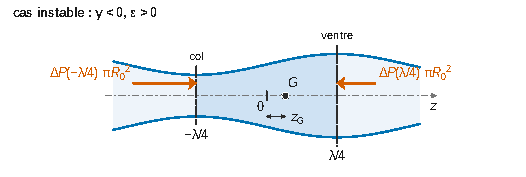
\includegraphics{figures/q19-q20-tranche-col-ventre.pdf}
\caption*{Figure 4 --- tranche de Q19-Q20 dans le cas instable : la surpression
plus forte au col pousse la tranche vers le ventre}
\end{figure}

La relation fondamentale appliquée au centre de gravité de la tranche, \(m\ddot z_G=F_z\), avec \(z_G=\sigma\lambda\varepsilon/R_0\), donne

\equationajustee{\mu\pi\frac{R_0^2\lambda}2\cdot\frac{\sigma\lambda}{R_0}\ddot\varepsilon=-8\pi R_0^2\alpha\gamma\varepsilon ,}

soit

\equationajustee{\ddot\varepsilon+\frac{16\alpha\gamma R_0}{\mu\sigma\lambda^2}\varepsilon=0 .}

On pose \(\xi=kR_0\). Alors \(\gamma=(\xi^2-1)/(4R_0^2)\), \(\lambda^2=4\pi^2R_0^2/\xi^2\) et \(\tau_h^2=\mu R_0^3/\alpha\) :

\equationajustee{\boxed{\ddot\varepsilon+\frac{\xi^2(\xi^2-1)}{\pi^2\sigma\,\tau_h^2}\,\varepsilon=0}}

Avec \(\sigma=2/\pi^2\), cette équation s'écrit

\equationajustee{\ddot\varepsilon+\frac{\xi^2(\xi^2-1)}{2\tau_h^2}\varepsilon=0 .}

\textbf{Discussion.}

\begin{itemize}
\tightlist
\item
  \(\xi>1\) (\(\lambda<2\pi R_0\)) : oscillateur harmonique de pulsation \(\omega=\dfrac{\xi\sqrt{\xi^2-1}}{\pi\sqrt\sigma\,\tau_h}\) ; \(\varepsilon\) reste bornée, la perturbation est \textbf{stable}.
\item
  \(\xi<1\) (\(\lambda>2\pi R_0\)) : \(\varepsilon(t)=a\,e^{t/\tau_k}+b\,e^{-t/\tau_k}\). Pour des conditions initiales génériques (\(a\neq0\)), \(\varepsilon\) diverge comme \(\exp(t/\tau_k)\) : \textbf{instable}.
\item
  \(\xi=1\) : cas marginal (\(\ddot\varepsilon=0\)).
\end{itemize}

On retrouve le critère de la question 16.

\textbf{Temps caractéristique} (cas \(\xi<1\)). On a \(1/\tau_k^2=\xi^2(1-\xi^2)/(\pi^2\sigma\tau_h^2)\), donc

\equationajustee{\boxed{\tau_k=\frac{\pi\sqrt\sigma\,\tau_h}{\xi\sqrt{1-\xi^2}}=\frac{\sqrt2\,\tau_h}{\xi\sqrt{1-\xi^2}}}}

\textbf{Minimum.} On pose \(u=\xi^2\in\,]0,1[\). \(\tau_k\) est minimal quand \(u(1-u)\) est maximal, c'est-à-dire en \(u=1/2\), où \(u(1-u)=1/4\). Donc \(\xi_c=1/\sqrt2\) et

\equationajustee{\boxed{\tau_{\min}=2\pi\sqrt\sigma\,\tau_h=2\sqrt2\,\tau_h}}

\equationajustee{\boxed{\lambda_c=\frac{2\pi R_0}{\xi_c}=2\sqrt2\,\pi R_0}}

Numériquement, \(\tau_{\min}\approx2{,}8\,\tau_h\) et \(\lambda_c\approx8{,}9\,R_0\).

\begin{figure}[H]
\centering
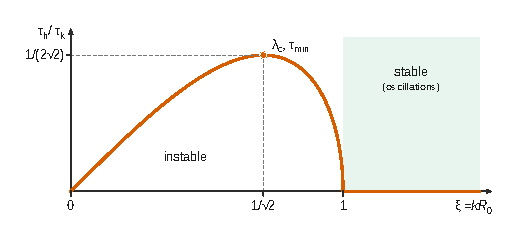
\includegraphics{figures/q20-taux-de-croissance.pdf}
\caption*{Figure 5 --- taux de croissance τ\_h/τ\_k = ξ√(1−ξ²)/√2 : nul au-delà de
ξ = 1, maximal en ξ\_c = 1/√2}
\end{figure}

\hypertarget{question-21}{%
\subsection{Question 21}\label{question-21}}

\textbf{Pourquoi \(\lambda_c\).} La perturbation réelle est un bruit qui contient toutes les longueurs d'onde. Le modèle étant linéaire, chaque composante de Fourier évolue indépendamment, et toutes celles de longueur d'onde supérieure à \(2\pi R_0\) croissent comme \(\exp(t/\tau_k)\).

Le rapport d'amplitude entre la composante \(\lambda_c\) et une autre croît comme \(\exp\big[t(1/\tau_{\min}-1/\tau_k)\big]\). Après quelques \(\tau_{\min}\), le mode \(\lambda_c\) domine et le jet se pince à ses cols, espacés de \(\lambda_c\). Il est donc raisonnable que le jet se coupe en tronçons de longueur \(\lambda_c\).

\textbf{Rayon des gouttes.} Un tronçon donne une goutte. Par conservation du volume :

\equationajustee{\tfrac43\pi R_g^3=\pi R_0^2\lambda_c=2\sqrt2\pi^2R_0^3 ,}

\equationajustee{\boxed{R_g=\left(\frac{3\pi}{\sqrt2}\right)^{1/3}R_0\approx1{,}9\,R_0}}

\textbf{Surfaces.} Avant fragmentation, \(S_{\rm cyl}=2\pi R_0\lambda_c=4\sqrt2\pi^2R_0^2\approx56\,R_0^2\). Après, \(S_{\rm sph}=4\pi R_g^2\approx44\,R_0^2\).

Plus directement, à volume \(V\) égal, \(S_{\rm cyl}=2V/R_0\) et \(S_{\rm sph}=3V/R_g\), donc

\equationajustee{\boxed{\frac{S_{\rm sph}}{S_{\rm cyl}}=\frac{3R_0}{2R_g}\approx0{,}8}}

La fragmentation \textbf{diminue l'aire de l'interface d'environ 20 \%}, donc l'énergie de surface \(\alpha S\) : l'évolution est énergétiquement favorable, en accord avec la question 16. Cette comparaison entre état initial et état final sort du cadre linéaire \(\varepsilon\ll R_0\) : c'est un argument de plausibilité, pas une démonstration.

\hypertarget{iv.b-expuxe9rience}{%
\subsection{IV.B Expérience}\label{iv.b-expuxe9rience}}

\hypertarget{question-22}{%
\subsection{Question 22}\label{question-22}}

Données : \(R_0=2\times10^{-3}\) m (le diamètre vaut \(4\) mm), \(v=1\ \mathrm{m\cdot s^{-1}}\), \(\alpha=7{,}2\times10^{-2}\ \mathrm{N\cdot m^{-1}}\).

\equationajustee{\tau_h=\sqrt{\frac{10^3\times8\times10^{-9}}{7{,}2\times10^{-2}}}\ \mathrm s=\sqrt{1{,}1\times10^{-4}}\ \mathrm s\approx1{,}05\times10^{-2}\ \mathrm s .}

\textbf{Distance de brisure.} La vitesse restant égale à \(v\), le jet se fragmente à la distance \(\ell=v\cdot10\tau_h\approx0{,}1\) m :

\equationajustee{\boxed{\ell\approx1\times10^{-1}\ \mathrm m}}

\textbf{Fréquence des chocs.} Une goutte se forme par longueur \(\lambda_c=2\sqrt2\pi R_0\approx1{,}8\times10^{-2}\) m de jet, qui défile à la vitesse \(v\). Les gouttes arrivent donc à l'évier à la cadence

\equationajustee{\boxed{f=\frac{v}{\lambda_c}=\frac{1}{1{,}8\times10^{-2}}\ \mathrm{Hz}\approx6\times10^1\ \mathrm{Hz}}}

C'est une fréquence audible (son grave), en accord avec l'observation.

\end{document}
